\section{Wetland model (model ID: 02)}
The Wetland model (fig.~\ref{fig:02_schematic}) is a conceptualization of the perceived dominant processes in a typical Western European wetland \citep{Savenije2010}. It belongs to a 3-part topography driven modelling exercise, together with a hillslope and plateau conceptualization. Each model is provided in isolation here, because they are well-suited for isolating specific model structure choices. It has 1 store and 4 parameters ($D_w$, $S_{w,max}$, $\beta_w$ and $K_w$). The model aims to represent:

\begin{itemizecompact}
\item Stylized interception by vegetation;
\item Evaporation;
\item Saturation excess runoff generated from a distribution of soil depths;
\item A linear relation between storage and slow runoff.
\end{itemizecompact}

\subsection{MARRMoT model name}
m\_02\_wetland\_4p\_1s \\

% Equations
\subsection{Model equations}

% Model layout figure
{ 																	% This ensures it doesn't warp text further down
\begin{wrapfigure}{l}{4cm}
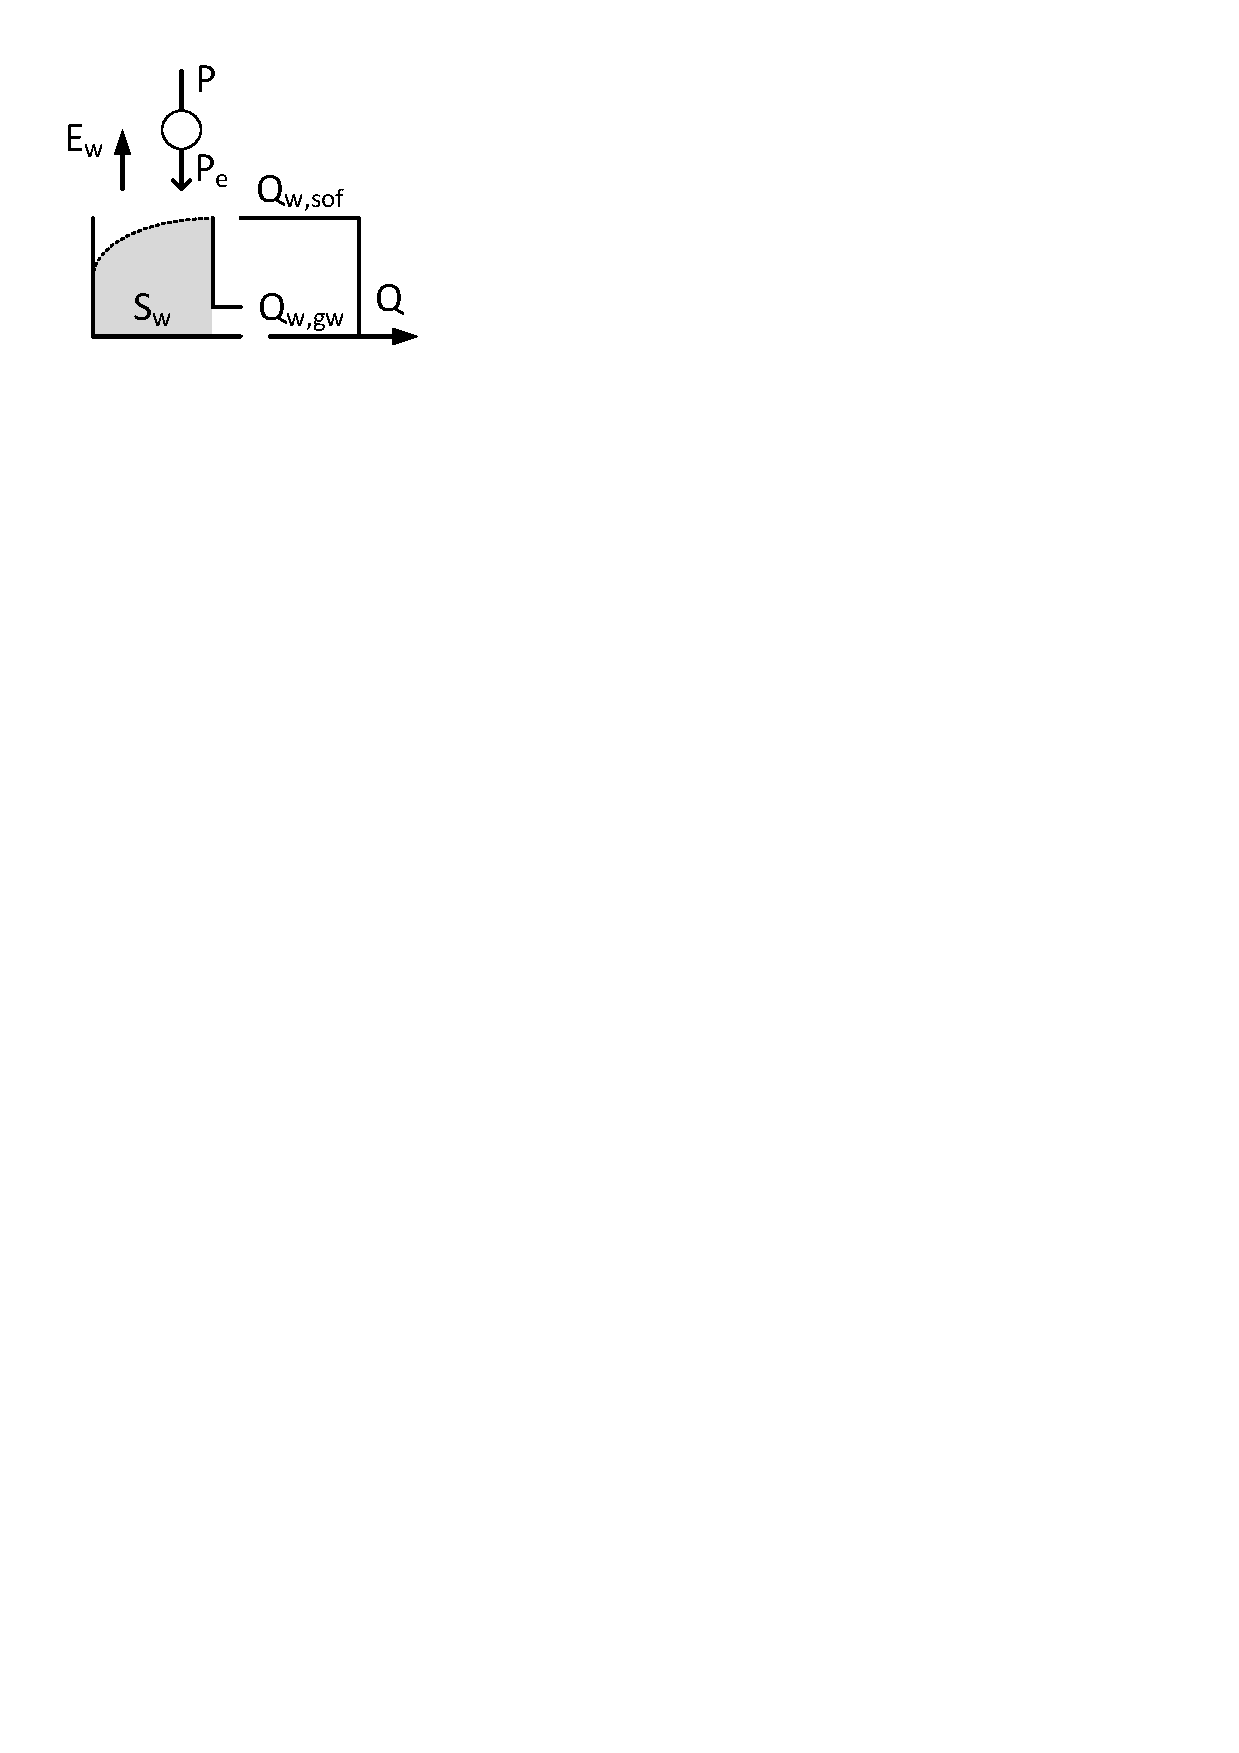
\includegraphics[trim=1cm 24cm 9cm 1cm,width=7cm,keepaspectratio]{./AppA_files/02_schematic.pdf}
\caption{Structure of the Wetland model} \label{fig:02_schematic}
\end{wrapfigure}

\begin{align}
	\frac{dS_w}{dt} &= P_e-E_w-Q_{w,sof}-Q_{w,gw} \\
	P_e &= max(P-D_w,0)\\
	E_w &= 
	\begin{cases}
		E_p, & \text{if } S_w > 0 \\
		0, & \text{otherwise}\\
	\end{cases}\\
	Q_{w,sof} &= \left(1-\left(1-\frac{S_w}{S_{w,max}}\right)^{\beta_w}\right)*P_e\\
	Q_{w,gw} &= K_w * S_w
\end{align}

} % end of wrapfigure fix

Where $S_w$ is the current soil water storage [mm]. Incoming precipitation P [mm/d] is reduced by interception $D_w$ [mm/d], which is assumed to evaporate before the next precipitation event. Evaporation from soil moisture $E_w$ [mm/d] occurs at the potential rate $E_p$ whenever possible. Saturation excess surface runoff $Q_{w,sof}$ [mm/d] depends on the fraction of the catchment that is currently saturated, expressed through parameters $S_{w,max}$ [mm] and $\beta_w$ [-]. Groundwater flow $Q_{w,gw}$ [mm/d] depends linearly on current storage $S_w$ through parameter $K_w$ [$d^{-1}$]. Total flow:

\begin{align}
	Q &= Q_{w,sof}+Q_{w,gw}
\end{align}

\newpage
\subsection{Parameter overview}
% Table generated by Excel2LaTeX from sheet 'Sheet1'
\begin{table}[htbp]
  \centering
    \begin{tabular}{lll}
    \toprule
    Parameter & Unit  & Description \\
    \midrule
    $D_w$ & $mm~d^{-1}$ & Interception evaporation  \\
    $S_{w,max}$ & $mm$  & Maximum soil moisture storage \\
    $\beta_w$ & $-$   & Non-linearity parameter for contributing area \\
    $K_w$ & $d^{-1}$ & Runoff coefficient \\
    \bottomrule
    \end{tabular}%
  \label{tab:addlabel}%
\end{table}%
